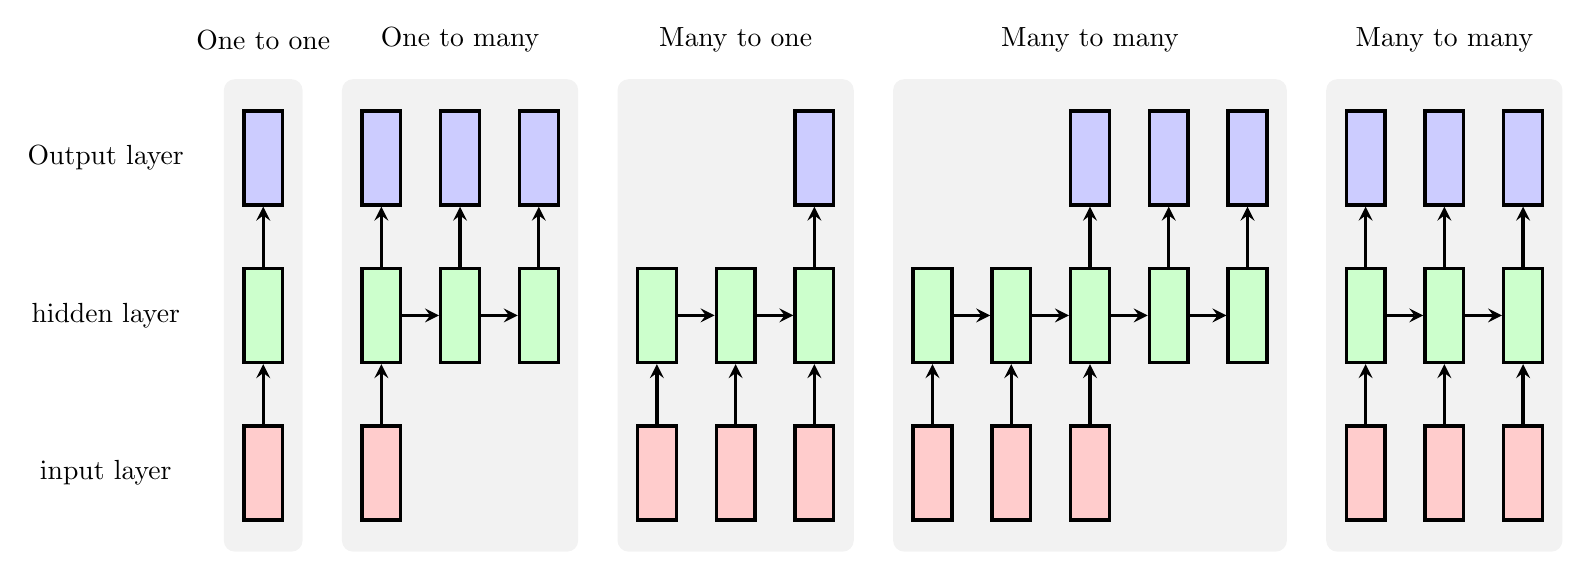
\begin{tikzpicture}
	\tikzstyle{input} = [draw,inner sep=7,minimum size=10,line 
	width=1, very thick, draw=black, fill=red!20, text width=20, text centered,rotate=90]
	\tikzstyle{hidden} = [draw,inner sep=7,minimum size=10,line 
	width=1, very thick, draw=black, fill=green!20, text width=20, text centered,rotate=90]
	\tikzstyle{output} = [draw,inner sep=7,minimum size=10,line 
	width=1, very thick, draw=black, fill=blue!20, text width=20, text centered,rotate=90]
	\tikzstyle{invisible} = [outer sep=0,inner sep=0,minimum size=0]
	\tikzstyle{stealth} = [-stealth, very thick]
	\fill [rounded corners, fill=gray!10] (-4,3.5) rectangle (-3,-2.5);
\fill [rounded corners, fill=gray!10] (-2.5,3.5) rectangle (0.5,-2.5);
\fill [rounded corners, fill=gray!10] (1,3.5) rectangle (4,-2.5);
\fill [rounded corners, fill=gray!10] (4.5,3.5) rectangle (9.5,-2.5);
\fill [rounded corners, fill=gray!10] (10,3.5) rectangle (13,-2.5);
\node [input] (v1) at (-3.5,-1.5) {};
\node [hidden] (v2) at (-3.5,0.5) {};
\node [output] (v3) at (-3.5,2.5) {};
\node [input] (v4) at (-2,-1.5) {};
\node [hidden] (v5) at (-2,0.5) {};
\node [hidden] (v7) at (-1,0.5) {};
\node [hidden] (v8) at (0,0.5) {};
\node [output] (v6) at (-2,2.5) {};
\node [output] (v9) at (-1,2.5) {};
\node [output] (v10) at (0,2.5) {};
\node [input] (v11) at (1.5,-1.5) {};
\node [input] (v13) at (2.5,-1.5) {};
\node [input] (v15) at (3.5,-1.5) {};
\node [hidden] (v12) at (1.5,0.5) {};
\node [hidden] (v14) at (2.5,0.5) {};
\node [hidden] (v16) at (3.5,0.5) {};
\node [output] (v17) at (3.5,2.5) {};
\node [input] (v18) at (5,-1.5) {};
\node [input] (v20) at (6,-1.5) {};
\node [input] (v22) at (7,-1.5) {};
\node [hidden] (v19) at (5,0.5) {};
\node [hidden] (v21) at (6,0.5) {};
\node [hidden] (v23) at (7,0.5) {};
\node [hidden] (v25) at (8,0.5) {};
\node [hidden] (v27) at (9,0.5) {};
\node [output] (v24) at (7,2.5) {};
\node [output] (v26) at (8,2.5) {};
\node [output] (v28) at (9,2.5) {};
\node [input] (v29) at (10.5,-1.5) {};
\node [input] (v32) at (11.5,-1.5) {};
\node [input] (v35) at (12.5,-1.5) {};
\node [hidden] (v30) at (10.5,0.5) {};
\node [hidden] (v33) at (11.5,0.5) {};
\node [hidden] (v36) at (12.5,0.5) {};
\node [output] (v31) at (10.5,2.5) {};
\node [output] (v34) at (11.5,2.5) {};
\node [output] (v37) at (12.5,2.5) {};
\draw [stealth] (v1) edge (v2);
\draw [stealth] (v2) edge (v3);
\draw [stealth] (v4) edge (v5);
\draw [stealth] (v5) edge (v6);
\draw [stealth] (v5) edge (v7);
\draw [stealth] (v7) edge (v8);
\draw [stealth] (v7) edge (v9);
\draw [stealth] (v8) edge (v10);
\draw [stealth] (v11) edge (v12);
\draw [stealth] (v13) edge (v14);
\draw [stealth] (v15) edge (v16);
\draw [stealth] (v12) edge (v14);
\draw [stealth] (v14) edge (v16);
\draw [stealth] (v16) edge (v17);
\draw [stealth] (v18) edge (v19);
\draw [stealth] (v20) edge (v21);
\draw [stealth] (v22) edge (v23);
\draw [stealth] (v23) edge (v24);
\draw [stealth] (v25) edge (v26);
\draw [stealth] (v27) edge (v28);
\draw [stealth] (v19) edge (v21);
\draw [stealth] (v21) edge (v23);
\draw [stealth] (v23) edge (v25);
\draw [stealth] (v25) edge (v27);
\draw [stealth] (v29) edge (v30);
\draw [stealth] (v30) edge (v31);
\draw [stealth] (v32) edge (v33);
\draw [stealth] (v33) edge (v34);
\draw [stealth] (v35) edge (v36);
\draw [stealth] (v36) edge (v37);
\draw [stealth] (v30) edge (v33);
\draw [stealth] (v33) edge (v36);

\node [invisible] at (-3.5,4) {One to one};
\node [invisible] at (-1,4) {One to many};
\node [invisible] at (2.5,4) {Many to one};
\node [invisible] at (7,4) {Many to many};
\node [invisible] at (11.5,4) {Many to many};
\node [invisible] at (-5.5,-1.5) {input layer};
\node [invisible] at (-5.5,0.5) {hidden layer};
\node [invisible] at (-5.5,2.5) {Output layer};
\end{tikzpicture}